\documentclass{standalone}
\usepackage{tikz}

\begin{document}
    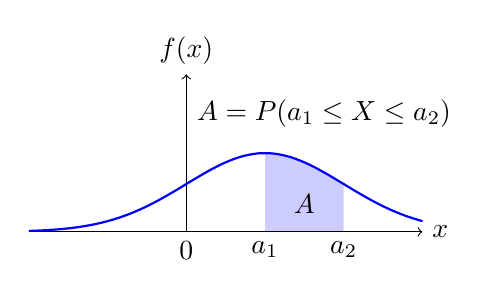
\begin{tikzpicture}
        
        % Draw and shade the area under the bell curve from x=1 to x=2
        \begin{scope}
            \fill[blue!20] 
            (1,0) -- plot[domain=1:2,smooth] (\x,{exp(-(\x-1)*(\x-1)/2)}) -- (2,0) -- cycle;
        \end{scope}
    
        \node at (1.5,0.35) {$A$};
        \node at (1.75,1.5) {$A=P(a_1 \leq X \leq a_2)$};

        % Draw the x and y axes
        \draw[->] (-2,0) -- (3,0) node[right] {$x$};
        \draw[->] (0,0) -- (0,2) node[above] {$f(x)$};

        % Draw the bell curve
        \draw[scale=1.0,domain=-2:3,smooth,variable=\x,blue,thick] 
            plot ({\x},{exp(-(\x-1)*(\x-1)/2)});
        
        % Optionally, add labels
        \node[below] at (0,0) {$0$};
        \node[below] at (1,0) {$a_1$};
        \node[below] at (2,0) {$a_2$};
    \end{tikzpicture}
\end{document}
